\section{Dispersive Readout}
\label{sec:readout}

The readout mechanism allows us to measure the state of the qubit in a non-demolishing way \cite{singleshot_readout}.
In our experiments this is needed in order to characterize the device and for calibration purposes.

The transmon our capacitively coupled to a readout resonator, which is a waveguide on our device.
By sending through this waveguide a signal far detuned from the qubit's frequency, its frequency will slightly change depending on the state of the qubit, without interfering with the state of the latter.
This process ids described by the James-Cummins Hamiltonian
\begin{equation}
    \hat{H} = \hbar \omega_r \hat{a}^\dagger \hat{a} + \frac{1}{2} \hbar \omega_{ge} \hat{\sigma}^z + \hbar g (\hat{a}^\dagger \hat{\sigma}^- + \hat{a} \hat{\sigma}^+) ,
\end{equation}
which models the coupling between a 2-level system and a light mode in a cavity.
Thus, by measuring the frequency shift of the readout resonator, we are able to infer the qubit's state.

In order to not let the qubit couple too strongly to the environment through the readout resonator, a Purcell filter is applied between the resonator and the qubit (see \cref{fig:diagram_storage_qubit}).
This allows to keep the lifetimes of the qubits longer, by suppressing spontaneous emission due to the Purcell effect \cite{Purcell_effect}.

\begin{figure}
    \centering
    

\tikzset{every picture/.style={line width=0.75pt}} %set default line width to 0.75pt      

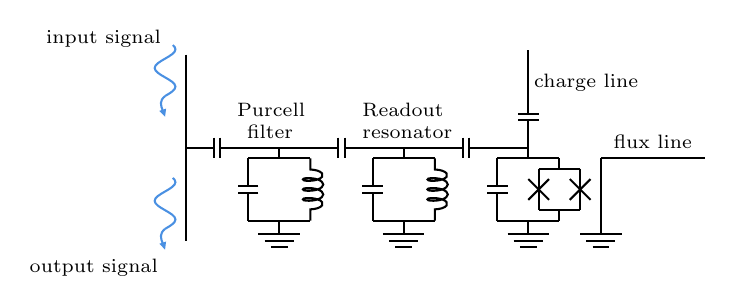
\begin{tikzpicture}[x=0.75pt,y=0.75pt,yscale=-1,xscale=1]
%uncomment if require: \path (0,300); %set diagram left start at 0, and has height of 300

%Shape: Capacitor [id:dp6229484510249941] 
\draw   (80,115) -- (93.5,115) (96.5,110) -- (96.5,120) (93.5,110) -- (93.5,120) (96.5,115) -- (110,115) ;
%Straight Lines [id:da5079772797363618] 
\draw    (140,120) -- (110,120) ;
%Shape: Inductor (Air Core) [id:dp10839806036975186] 
\draw   (140,120) -- (140,125.4) .. controls (142.63,125.48) and (144.87,126.23) .. (145.66,127.29) .. controls (146.44,128.35) and (145.61,129.5) .. (143.55,130.2) .. controls (141.95,130.74) and (139.88,130.95) .. (137.87,130.8) .. controls (137.08,130.8) and (136.45,130.53) .. (136.45,130.2) .. controls (136.45,129.87) and (137.08,129.6) .. (137.87,129.6) .. controls (139.88,129.45) and (141.95,129.66) .. (143.55,130.2) .. controls (145.26,130.82) and (146.23,131.69) .. (146.23,132.6) .. controls (146.23,133.51) and (145.26,134.38) .. (143.55,135) .. controls (141.95,135.54) and (139.88,135.75) .. (137.87,135.6) .. controls (137.08,135.6) and (136.45,135.33) .. (136.45,135) .. controls (136.45,134.67) and (137.08,134.4) .. (137.87,134.4) .. controls (139.88,134.25) and (141.95,134.46) .. (143.55,135) .. controls (145.26,135.62) and (146.23,136.49) .. (146.23,137.4) .. controls (146.23,138.31) and (145.26,139.18) .. (143.55,139.8) .. controls (141.95,140.34) and (139.88,140.55) .. (137.87,140.4) .. controls (137.08,140.4) and (136.45,140.13) .. (136.45,139.8) .. controls (136.45,139.47) and (137.08,139.2) .. (137.87,139.2) .. controls (139.88,139.05) and (141.95,139.26) .. (143.55,139.8) .. controls (145.61,140.5) and (146.44,141.65) .. (145.66,142.71) .. controls (144.87,143.77) and (142.63,144.52) .. (140,144.6) -- (140,150) ;
%Shape: Capacitor [id:dp06818692783071034] 
\draw   (110,120) -- (110,133.5) (115,136.5) -- (105,136.5) (115,133.5) -- (105,133.5) (110,136.5) -- (110,150) ;
%Straight Lines [id:da7350026547264685] 
\draw    (110,150) -- (140,150) ;
%Straight Lines [id:da23995913734624486] 
\draw    (80,70) -- (80,160) ;
%Straight Lines [id:da1612492392898659] 
\draw    (110,115) -- (140,115) ;
%Straight Lines [id:da5671640840709973] 
\draw    (125,115) -- (125,120) ;
%Shape: Capacitor [id:dp5438650003798182] 
\draw   (140,115) -- (153.5,115) (156.5,110) -- (156.5,120) (153.5,110) -- (153.5,120) (156.5,115) -- (170,115) ;
%Straight Lines [id:da49049414599623864] 
\draw    (200,120) -- (170,120) ;
%Shape: Inductor (Air Core) [id:dp010409349579149074] 
\draw   (200,120) -- (200,125.4) .. controls (202.63,125.48) and (204.87,126.23) .. (205.66,127.29) .. controls (206.44,128.35) and (205.61,129.5) .. (203.55,130.2) .. controls (201.95,130.74) and (199.88,130.95) .. (197.87,130.8) .. controls (197.08,130.8) and (196.45,130.53) .. (196.45,130.2) .. controls (196.45,129.87) and (197.08,129.6) .. (197.87,129.6) .. controls (199.88,129.45) and (201.95,129.66) .. (203.55,130.2) .. controls (205.26,130.82) and (206.23,131.69) .. (206.23,132.6) .. controls (206.23,133.51) and (205.26,134.38) .. (203.55,135) .. controls (201.95,135.54) and (199.88,135.75) .. (197.87,135.6) .. controls (197.08,135.6) and (196.45,135.33) .. (196.45,135) .. controls (196.45,134.67) and (197.08,134.4) .. (197.87,134.4) .. controls (199.88,134.25) and (201.95,134.46) .. (203.55,135) .. controls (205.26,135.62) and (206.23,136.49) .. (206.23,137.4) .. controls (206.23,138.31) and (205.26,139.18) .. (203.55,139.8) .. controls (201.95,140.34) and (199.88,140.55) .. (197.87,140.4) .. controls (197.08,140.4) and (196.45,140.13) .. (196.45,139.8) .. controls (196.45,139.47) and (197.08,139.2) .. (197.87,139.2) .. controls (199.88,139.05) and (201.95,139.26) .. (203.55,139.8) .. controls (205.61,140.5) and (206.44,141.65) .. (205.66,142.71) .. controls (204.87,143.77) and (202.63,144.52) .. (200,144.6) -- (200,150) ;
%Shape: Capacitor [id:dp38289405277156474] 
\draw   (170,120) -- (170,133.5) (175,136.5) -- (165,136.5) (175,133.5) -- (165,133.5) (170,136.5) -- (170,150) ;
%Straight Lines [id:da7342631646168638] 
\draw    (170,150) -- (200,150) ;
%Shape: Capacitor [id:dp4965705456609162] 
\draw   (200,115) -- (213.5,115) (216.5,110) -- (216.5,120) (213.5,110) -- (213.5,120) (216.5,115) -- (230,115) ;
%Straight Lines [id:da5477595668599946] 
\draw    (170,115) -- (200,115) ;
%Straight Lines [id:da7609436744451872] 
\draw    (185,115) -- (185,120) ;
%Straight Lines [id:da932132356010352] 
\draw    (260,120) -- (230,120) ;
%Shape: Capacitor [id:dp925083204210299] 
\draw   (230,120) -- (230,133.5) (235,136.5) -- (225,136.5) (235,133.5) -- (225,133.5) (230,136.5) -- (230,150) ;
%Straight Lines [id:da48756322841661204] 
\draw    (230,150) -- (260,150) ;
%Straight Lines [id:da9662762169593431] 
\draw    (245,115) -- (245,120) ;
%Straight Lines [id:da607486087129423] 
\draw    (250,125) -- (270,125) ;
%Straight Lines [id:da4269839144692542] 
\draw    (250,145) -- (270,145) ;
%Straight Lines [id:da6212379775483154] 
\draw    (270,125) -- (270,145) ;
%Straight Lines [id:da42941601462568646] 
\draw    (250,125) -- (250,145) ;
%Straight Lines [id:da9671029825944342] 
\draw    (260,120) -- (260,125) ;
%Straight Lines [id:da9712181495027408] 
\draw    (260,145) -- (260,150) ;
%Straight Lines [id:da3624697790998732] 
\draw    (265,130) -- (275,140) ;
%Straight Lines [id:da4335724022567018] 
\draw    (245,130) -- (255,140) ;
%Straight Lines [id:da530417781084312] 
\draw    (255,130) -- (245,140) ;
%Straight Lines [id:da9581131846208597] 
\draw    (275,130) -- (265,140) ;
%Straight Lines [id:da038301723534536425] 
\draw    (230,115) -- (245,115) ;
%Shape: Ground [id:dp6910953506421662] 
\draw   (115,156.67) -- (135,156.67) ;
\draw   (118,159.67) -- (132,159.67) ;
\draw   (121,162.67) -- (129,162.67) ;
\draw   (125,150) -- (125,156.67) ;
%Shape: Ground [id:dp4840755871676472] 
\draw   (175,156.67) -- (195,156.67) ;
\draw   (178,159.67) -- (192,159.67) ;
\draw   (181,162.67) -- (189,162.67) ;
\draw   (185,150) -- (185,156.67) ;
%Shape: Ground [id:dp7159028270026297] 
\draw   (235,156.67) -- (255,156.67) ;
\draw   (238,159.67) -- (252,159.67) ;
\draw   (241,162.67) -- (249,162.67) ;
\draw   (245,150) -- (245,156.67) ;
%Straight Lines [id:da07274023253816075] 
\draw    (280,120) -- (330,120) ;
%Straight Lines [id:da0646328748380458] 
\draw    (280,120) -- (280,150) ;
%Shape: Ground [id:dp10990759893272828] 
\draw   (270,156.67) -- (290,156.67) ;
\draw   (273,159.67) -- (287,159.67) ;
\draw   (276,162.67) -- (284,162.67) ;
\draw   (280,150) -- (280,156.67) ;
%Straight Lines [id:da8443452176258857] 
\draw    (245,68) -- (245,85) ;
%Shape: Capacitor [id:dp2673784375807502] 
\draw   (245,85) -- (245,98.5) (250,101.5) -- (240,101.5) (250,98.5) -- (240,98.5) (245,101.5) -- (245,115) ;
%Shape: Wave [id:dp46962992426174544] 
\draw  [color={rgb, 255:red, 74; green, 144; blue, 226 }  ,draw opacity=1 ] (70,90) .. controls (72.56,88.53) and (75,87.13) .. (75,85.5) .. controls (75,83.87) and (72.56,82.47) .. (70,81) .. controls (67.44,79.53) and (65,78.13) .. (65,76.5) .. controls (65,74.87) and (67.44,73.47) .. (70,72) .. controls (72.56,70.53) and (75,69.13) .. (75,67.5) .. controls (75,66.77) and (74.51,66.09) .. (73.75,65.43) ;
%Curve Lines [id:da8193635142444085] 
\draw [color={rgb, 255:red, 74; green, 144; blue, 226 }  ,draw opacity=1 ]   (70,90) .. controls (67.21,92.34) and (67.82,94.25) .. (68.96,97.21) ;
\draw [shift={(70,100)}, rotate = 251.57] [fill={rgb, 255:red, 74; green, 144; blue, 226 }  ,fill opacity=1 ][line width=0.08]  [draw opacity=0] (3.57,-1.72) -- (0,0) -- (3.57,1.72) -- cycle    ;
%Shape: Wave [id:dp5292058745377288] 
\draw  [color={rgb, 255:red, 74; green, 144; blue, 226 }  ,draw opacity=1 ] (70,154) .. controls (72.56,152.53) and (75,151.13) .. (75,149.5) .. controls (75,147.87) and (72.56,146.47) .. (70,145) .. controls (67.44,143.53) and (65,142.13) .. (65,140.5) .. controls (65,138.87) and (67.44,137.47) .. (70,136) .. controls (72.56,134.53) and (75,133.13) .. (75,131.5) .. controls (75,130.77) and (74.51,130.09) .. (73.75,129.43) ;
%Curve Lines [id:da04097203302843688] 
\draw [color={rgb, 255:red, 74; green, 144; blue, 226 }  ,draw opacity=1 ]   (70,154) .. controls (67.21,156.34) and (67.82,158.25) .. (68.96,161.21) ;
\draw [shift={(70,164)}, rotate = 251.57] [fill={rgb, 255:red, 74; green, 144; blue, 226 }  ,fill opacity=1 ][line width=0.08]  [draw opacity=0] (3.57,-1.72) -- (0,0) -- (3.57,1.72) -- cycle    ;

% Text Node
\draw (305,117) node [anchor=south] [inner sep=0.75pt]  [font=\scriptsize] [align=left] {{\scriptsize flux line}};
% Text Node
\draw (246.31,83.64) node [anchor=west] [inner sep=0.75pt]  [font=\scriptsize] [align=left] {{\scriptsize charge line}};
% Text Node
\draw (181,112) node [anchor=south] [inner sep=0.75pt]  [font=\scriptsize] [align=left] {\begin{minipage}[lt]{23.84pt}\setlength\topsep{0pt}
\begin{center}
{\scriptsize Readout}\\{\scriptsize resonator }
\end{center}

\end{minipage}};
% Text Node
\draw (138,112) node [anchor=south east] [inner sep=0.75pt]  [font=\scriptsize] [align=left] {\begin{minipage}[lt]{23.84pt}\setlength\topsep{0pt}
\begin{center}
{\scriptsize Purcell}\\{\scriptsize filter}
\end{center}

\end{minipage}};
% Text Node
\draw (69.47,67.86) node [anchor=south east] [inner sep=0.75pt]  [font=\scriptsize] [align=left] {{\scriptsize input signal}};
% Text Node
\draw (68,167) node [anchor=north east] [inner sep=0.75pt]  [font=\scriptsize] [align=left] {{\scriptsize output signal}};


\end{tikzpicture}


    \vspace{-1cm}
    \caption{Diagram representing a storage qubit and their readout mechanism}
    \label{fig:diagram_storage_qubit}
\end{figure}
